\chapter{Architecture}

\section{System Overview}
Basically, the architecture consists of two main components namely the broker and
the client, whereas the client can act as producer, consumer or both. The broker
is a server which only reacts to requests that are sent from clients. Every
request contains an API key which the broker uses to determine which action it
has to do (e.g. persist produced message or consume message). For each valid
request the broker sends back a corresponding response to the client which
either includes the fetched data or an error code. The broker never communicates
with a client without a request.

\begin{figure}[H]
    \centering
     \begin{sequencediagram}
        %\newthread{broker}{Broker}
         \newinst[3]{client}{Client}
         \newinst[3]{broker}{Broker}
        \begin{messcall}
            {client}{(1) Send Request}{broker}{}
        \end{messcall}
        \begin{messcall}
            {broker}{(2) Do Action}{broker}{}
        \end{messcall}
        \begin{messcall}
            {broker}{(3) Send Response}{client}{} 
        \end{messcall}
     \end{sequencediagram}
     \caption{Basic communication between client (producer or consumer) and
     broker}
\end{figure}

\section{Prototype}
For demonstrating the architecture of this project we implement an architecture
prototype which shows basic functionality of producing a message from a client A
omplete) a  topic specific log at the broker and in turn consuming it from another
client B. It fully implements the produce and fetch request with their
appropriate responses of the Kafka protocol for communication over network.
Therefore the producer and consumer clients are compatible with original Apache
Kafka broker.

The functionality of the architecture prototype can be split in two cases.
Case one covers producing a message and persisting in the brokers log:
\begin{figure}[H]
    \centering
    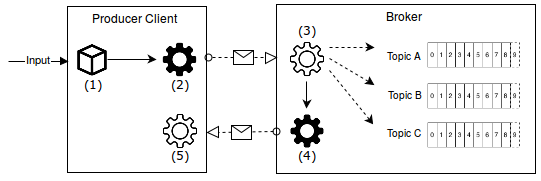
\includegraphics[width=0.8\textwidth]{images/concept_producer.png}
    \caption{Concept of Architecture Prototype Part I}
    \label{fig:conept-producer}
\end{figure}

\begin{table}[h]
\begin{tabular}{ll}
1  & Packing input message in data structure                                                          \\
2  & Serializing of data structure to byte string. The algorithm implements the Kafka protocol.       \\
3 & Transmitting byte string via TCP socket over network                                             \\
4  & Receiving and parsing byte string back to data structure                                         \\
5   & Write Message into topic specific log. The resulting file has same structure than the Kafka Log has.
\end{tabular}
\end{table}

Case two covers the part of consuming from a specific topic. Because Kafka works with 
pull-based consumption, the consumer fetch its messages with a constantly requesting it. 

\begin{figure}[H]
    \centering
   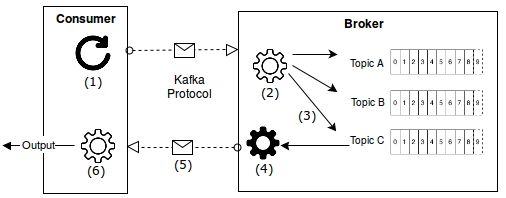
\includegraphics[width=0.7\textwidth]{images/concept_consumer.png}
    \caption{Concept of Architecture Prototype Part II}
    \label{fig:concept-consumer}
\end{figure}

\begin{table}[h]
\begin{tabular}{ll}
1  & Continuously send fetch request to broker implementing Kafka protocol \\
2  & Parse fetch request to data structure                                 \\
3  & Read messages from log of specified topic                             \\
4  & Serialize messages as response into byte string.                      \\
5  & Transmitting byte string back to consumer                             \\
6  & Parse response from broker to get messages                           
\end{tabular}
\end{table}

\section{Design decisions}
\subsection{Protocol}
For communicating over network we implement a binary protocol based on tcp.
Because we use Apache Kafka as benchmark for this project and we want to provide
compatibility to existing Kafka clients, we decided to fully implement the Kafka
Protocol version 0.8.x \todo{ref}. It differ in six APIs which each of it is
defined with a request-response message pair. The client initiates a socket connection and then
writes a sequence of request messages and reads back the corresponding response
message. 

\subsection{Separation} 
Both, the client and broker component need to use the same underlying protocol for
communication. Therefore we provide a third component which fully implements the Apache Kafka
protocol \todo{ref} and provides the appropriate functions and types as library.
This component fully separates the clients from the broker. It also allows to
use the clients with other Kafka based broker implementations, especially Apache
Kafka itself. 

A broker system should have as many client implementations as possible to
support interoperability. As basic clients a simple console-producer and
console-consumer is provided. To support the development of other clients a
another component which act as common client api is introduced. It provides
common functionality to simplify the use of the protocol implementation. 

\begin{figure}[H]
    \centering
    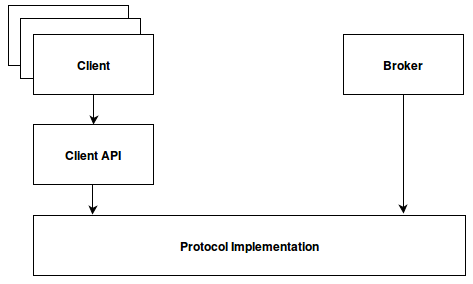
\includegraphics[width=0.55\textwidth]{images/architecture-components.png}
    \caption{Separation of code}
    \label{fig:architecture-components.png}
\end{figure}



%\section{Packages, Modules and Dependencies}
%\todo[inline]{how did we structure the executables ans libraries}
 
%The application has three main parts namely the broker, protocol implementation
%and the client api. 
%Each part is built in its own self-contained cabal package.

%\begin{figure}[H]
%    \centering
%   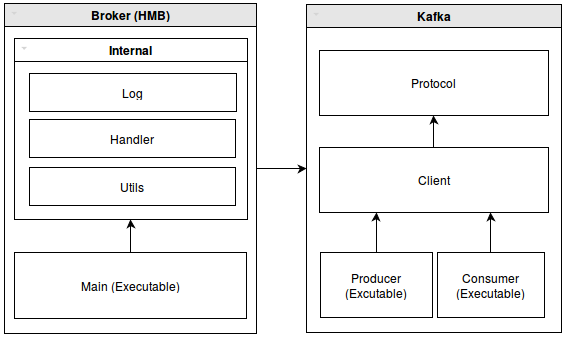
\includegraphics[width=0.7\textwidth]{images/logical-architecture.png}
%    \caption{Package structure and dependencies}
%    \label{fig:logical-architecture}
%\end{figure}

%\subsection{Protocol Implementation}


%\subsection{Encode / Decode}

%\subsection{Client (API)}

\section{Error Handling}

\section{Testing}
hspec 

\section{Client Examples}
This example shows a very basic console client which either can act as producer
by sending a producer request or as a consumer by sending a fetch request. After
sending the client wait for a corresponding response from the broker.

Init stream socket an open connection to a given host address and port (broker must be running on same ip and port): 
\begin{lstlisting}
  sock <- socket AF_INET Stream defaultProtocol 
  setSocketOption sock ReuseAddr 1
  putStrLn "Give IP"
  ipInput <- getLine
  let ip = toHostAddress (read ipInput :: IPv4)
  putStrLn "Give Port"
  port <- getLine
  connect sock (SockAddrInet port ip)
\end{lstlisting}
\todo{port convertierung}

If connection succeeded give client id and topic name: 
\begin{lstlisting}
  putStrLn "Give Client Id"
  clientId <- getLine
  putStrLn "Give Topic Name"
  topicName <- getLine
\end{lstlisting}

Producer: Sends given message to the broker. Client API function packPrRqMessage
packs the input into a protocol conform produce request, whereas the function
sendRequest encodes the request an send it over given socket connection.
Afterwards a response from broker is expected. If there is a response the client
can decode it with the API function decodePrResponse. 
\begin{lstlisting}
  forever $  do 
    putStrLn "Nachricht eingeben"
    inputMessage <- getLine
    sendRequest sock $ packPrRqMessage (clientId, topicName, 0, inputMessage)

    input <- recv sock 4096
    let response = decodePrResponse input
    print response 
\end{lstlisting}

Consumer: Send a fetch request with given offset to the broker. Analog to the producer request 
the api function packFtRqMessage packs the input into a protocol conform fetch request and sendRequest passes it via socket to the broker. 
\todo{code not final yet}


